\documentclass[11pt,pdftex,portrait,letterpaper]{article}
\usepackage[hdivide={1in,*,1in},
            vdivide={1in,*,1in},
%            showframe
            ]{geometry}

\usepackage{graphicx}
\usepackage{longtable}
\usepackage{acronym}
\usepackage{verbatim}
\usepackage{subfigure}
\usepackage{fancyhdr}
\pagestyle{fancy}
\usepackage{listings}
\usepackage{color}
\usepackage{lastpage}

% Default margins are too wide all the way around. Reset them here
\setlength{\topmargin}{-.5in}
\setlength{\textheight}{9in}
\setlength{\oddsidemargin}{.125in}
\setlength{\textwidth}{6.25in}

\lhead{ECEN 898}
\chead{}
\rhead{\thepage\ of \pageref{LastPage}}
%\lfoot{\hline}
\lfoot{}
\cfoot{\small{University of Nebraska - Lincoln Department of Electrical Engineering}}
\rfoot{}
\renewcommand{\footrulewidth}{0.5pt}


% Modify parameters of Listings
\lstset{ 
language=C,
basicstyle=\scriptsize,
numbers=left,
numberstyle=\footnotesize,
stepnumber=1,
numbersep=10pt,
backgroundcolor=\color{white},
frame=single,
captionpos=b,
breaklines=true,
breakatwhitespace=false
}

\begin{document}

\vspace*{30ex}
\begin{center}

\textbf{Project 05 - FFT LCD Display }\\

\vspace{4ex}
Introduction to Embedded Systems - University of Nebraska \\

\vspace{4ex}
Zach Swanson\\

\end{center}


\pagebreak
\tableofcontents
%\pagebreak
%\listoffigures
%\addcontentsline{toc}{section}{{\bf List of Figures}}
\pagebreak


\section{Introduction}

The purpose of this project was to introduce the fast Fourier transform (FFT) using the TI eZDSP5535 development board (eZDSP). A 256-point FFT was implemented for this project. The project required the use of BIOS to perform the operations of receiving audio, filtering audio, performing the FFT on the filtered audio signal, transmitting the filtered audio, and displaying the results of the FFT to the LCD display. Emphasis was placed on the quality of the project demonstration, i.e. sound and display quality. In order to achieve a quality display, a key challenge for this project was improving the frame rate for writing to the display.
 
\section{Project Description}

\subsection{Filter Design}

As in past projects, a low- and a high-pass filter were designed and implemented for filtering audio samples.  The cutoff frequency of both filters were increased to provide a larger range of frequencies for demonstrating the display for low frequency tones. The filters' magnitude responses are shown in Figure \ref{f:fig1}. Both filters were 127th order.

\begin{figure}[h]
\centering
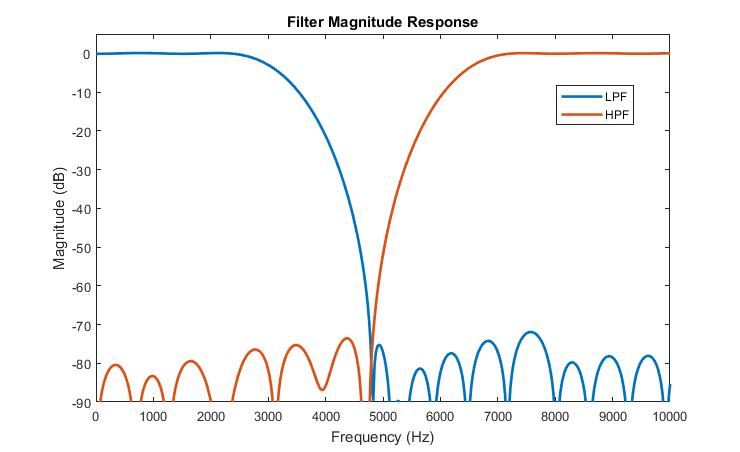
\includegraphics[width=0.8\textwidth]{./filtMag}
\caption{Magnitude response of low- and high-pass filters}
\label{f:fig1}
\end{figure}

\subsection{Program Description}

\subsubsection {Audio Handling}
The program contained two hardware interrupts, two tasks, two idle threads and two mailboxes. Figure \ref{f:fig2} illustrates the overall flow of the program in a block diagram. Audio was sampled at a rate of 48 kHz by the stereo-in ADC. The I2S receive hardware interrupt was used to collect samples using a ping-pong array. Every 48 samples collected, the hardware interrupt posted the samples to a mailbox. The mailbox, MBXAudio, featured two messages, each containing 48 elements. The mailbox was read by the audio filtering task. The task execution was suspended until a message was available; then, the samples were dumped into an array that was passed to a previously designed FIR filter function. The FIR function output the filtered audio samples to another ping-pong array. The ping-pong array was read by the I2S transmit hardware interrupt, which fed the filtered samples to the stereo-out DAC to play the audio to the listener. The transmit ping-pong array elements were also copied to an array to be passed to a second task that performed the FFT.  

\begin{figure}[h]
\centering
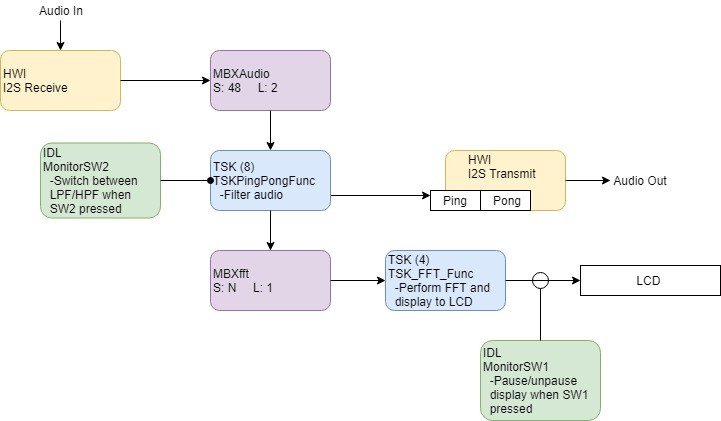
\includegraphics[width=0.8\textwidth]{./blocks}
\caption{Block diagram of program flow.}
\label{f:fig2}
\end{figure}

\subsubsection {FFT Calculation}
The FFT is a transform that takes a discrete time signal and generates the signals frequency response. It is defined as being an "N-point" transform, where N is the number of frequency bins generated by the transform. The FFT output may also be defined by the window size, L, of the input data. For simplicity, N and L were kept equal to each other throughout the project, such that the computational and frequency resolution were always equal. 

The rfft function from the TI-provided DSP library was used to implement the FFT in this program. To perform a N-point FFT, the rfft function required N data samples. Therefore, the audio filtering task had to copy N filtered samples before posting to a second mailbox, MBXfft, that consisted of one message compromised of N elements. Similar to the filtering task, the FFT task was suspended until a message was available. Once a message was received, the rfft function was called. The rfft function generated complex output in the input data array; hence, the function generated half the output of a N-point FFT. However, only half of the output was needed because the FFT is a symmetric function around the Nyquist freqency. Because the output was in complex format the magnitude of the frequency spectrum was calculated. Listing \ref{l:code1} shows the the rfft call and the calculation of the magnitude response.

For this project, a 256-point FFT was performed. The value 256 was selected because the rfft function generated 128 output data points. Therefore, at 128 points, the entire 96 pixel columns of the LCD display could be utilized to display the majority of the frequency spectrum. 

\begin{lstlisting}[caption={FFT and magnitude calculation}, label=l:code1]
MBX_pend(&MBXfft, &data1, SYS_FOREVER);
max = 0;
rfft(data1, N, SCALE);

fftMag[0] = (int16_t)(sqrt( pow((double)(data1[0]), 2) ) );
fftMag[NBY2] = (int16_t)(sqrt( pow((double)(data1[1]), 2) ) );

for(i = 1, j = 2; i < NBY2; i++, j += 2)
{
	fftMag[i] = (int16_t)(sqrt( pow((double)(data1[j]), 2) + pow((double)(data1[(j + 1)]), 2) ) );

	if(fftMag[i] > max)
	{
		max = fftMag[i];
	}
}

IDL_run();
if(!displayFreeze)
{
	fftDisplay(fftMag, NBY2, max);
}
\end{lstlisting}

\subsubsection {FFT LCD Display}
After the FFT and the magnitude response were calculated, the magnitude data was passed to a function that calculated pixel position and wrote the positions to the LCD display. As Listing \ref{l:code1} shows, a maximum value was determined and passed to the display function. This was done to ensure that the magnitude display could be easily seen regardless of the relative magnitudes of different sample sets. Listing \ref{l:code2} shows the code for the function that wrote the FFT magnitude data to the display and \ref{l:code3} shows the TI multi-send command for the LCD display. As shown, the fftDisplay function used the same I2C\_write function as TI's multi-send function, but fftDisplay reduced the wait time by a factor of 100 which helped improve frame rates. Another frame rate improvement method was changing the addressing mode to vertical addressing mode, which wrote to the top and bottom page of the screen while moving horizontally across the screen. 

\begin{lstlisting}[caption={LCD display function}, label=l:code2]
void fftDisplay(int16_t * samples, int numSamps, int16_t maxVal)
{
	int i, j;
	Uint16 bot, top, cmd[193];

	cmd[0] = 0x40 & 0x00FF;

	for(i = 0, j = 1; i < 96; i++, j+=2)
	{
		pixLoc(samples[i], &bot, &top, maxVal);

		cmd[j] = bot;
		cmd[(j + 1)] = top;
	}

	EZDSP5535_waitusec( 10 );
	EZDSP5535_I2C_write(0x3C, &cmd[0], 193);
}
\end{lstlisting}

\begin{lstlisting}[caption={TI LCD multi-send function}, label=l:code3]
Int16 EZDSP5535_OSD9616_multiSend( Uint16* data, Uint16 len )
{
    Uint16 x;
    Uint16 cmd[10];
    for(x=0;x<len;x++)               // Command / Data
    {
    	cmd[x] = data[x];
    }
    EZDSP5535_waitusec( 1000 );
    return EZDSP5535_I2C_write( OSD9616_I2C_ADDR, cmd, len );
}
\end{lstlisting}

\subsubsection {Idle Threads}
As in previous projects, two idle threads were used to monitor switch one and two strokes. Similar to past projects, whenever a switch two stroke occurred the audio filter was switched from low- to high-pass or vice-versa. When a switch one stroke was detected, a state variable, displayFreeze, was changed to pause or unpause the display. Listing \ref{l:code1} shows how the state variable was used to control the LCD display. 

\section{Results}

\subsection{Display}

The best frame rate achieved was approximately 53 frames per second. As stated previously, the frame rates were improved by drastically reducing the time waiting before the I2C\_write call and by switching to vertical addressing mode. Additionally, to enhance the demo the pixels from the axis of the LCD graph to the actual data value pixel were illuminated to provided a better magnitude profile for the viewer. The only drawback of the screen was the screen provided 96 pixels along the x-axis. However, by performing a 256-point FFT, 128 pixels were needed to represent the positive frequency spectrum from DC to Nyquist. Hence, the screen in the demo displayed frequencies from zero to 18 kHz. Since the audio used for the demo would not likely exceed the upper bound, it was deemed acceptable.

\subsection{FFT Results}

Figures \ref{f:fig3} and \ref{f:fig4} show a comparison of the MATLAB and TI FFT results for the same input at 1,125 Hz and 5,000 Hz, respectively. As illustrated, the TI rfft results were similar to the MATLAB fft results, especially for the 1,125 Hz tone. The FFT on the 1,125 Hz tone was better for both FFT implementations because of the frequency resolution, which was equal to 187.5 Hz. Because 1,125 is a multiple of 187.5, it lines up with one of the transform output bins. On the other hand, the 5,000 Hz tone was not a multiple of 187.5 and spreading of frequency near 5,000 Hz was observed as a result. It was also observed that the peak wasn't exactly at 5,000; rather, it was shifted to the next nearest multiple of 187.5 Hz, 5,062.5 Hz.

\begin{figure}[h]
\centering
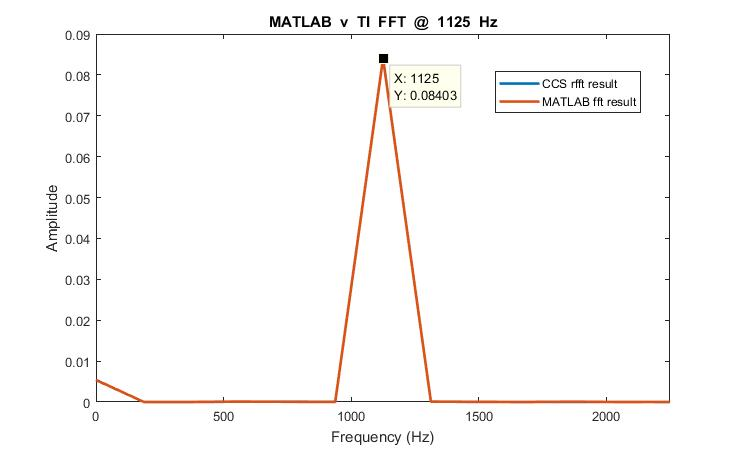
\includegraphics[width=0.8\textwidth]{./1125Compare}
\caption{MATLAB and CCS comparison of FFT results at 1125 Hz Tone}
\label{f:fig3}
\end{figure}

\begin{figure}[h]
\centering
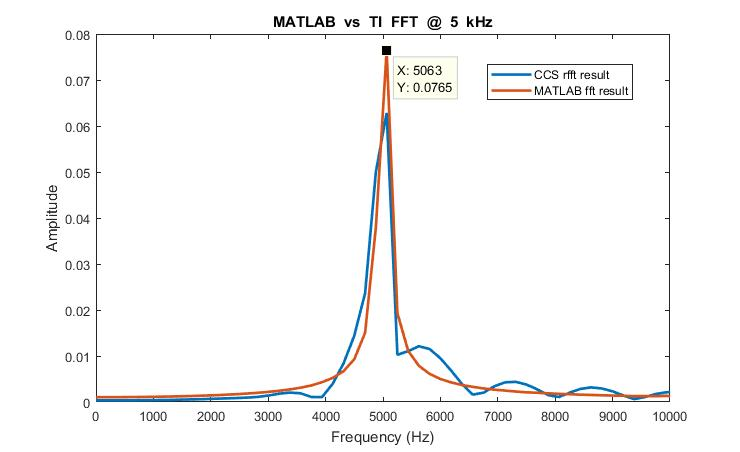
\includegraphics[width=0.8\textwidth]{./5kCompare}
\caption{MATLAB and CCS comparison of FFT results at 5000 Hz Tone}
\label{f:fig4}
\end{figure}

\subsection{CPU Usage}
To accurately measure the CPU usage of the tasks the HWI\_disable/HWI\_restore and TSK\_disable/TSK\_enable commands were used to suspend unwanted hardware interrupts and tasks. For the audio sampling task, the cycles were counted from one mailbox pend to the next. The audio sampling task takes 12,032 cycles when using a 128 coefficient filter. Filtering 48-sample frames, the CPU usage for the task was 12\%. For the FFT task, the cycles were counted from the mailbox pend to a dummy line of code at the end of the task. The FFT task took 3,019,811 cycles to complete. Hence, when the task was running, it was consuming 100\% of the CPU time. Therefore, the task was given lowest priority, no other tasks or hardware interrupts depended on the FFT task and the IDL\_run command was called within the task to ensure the idle threads were called.

\pagebreak

\section{Appendix}

\begin{lstlisting}[caption={main.c}, label=l:program1]
/*
 *  Copyright 2010 by Texas Instruments Incorporated.
 *  All rights reserved. Property of Texas Instruments Incorporated.
 *  Restricted rights to use, duplicate or disclose this code are
 *  granted through contract.
 *
 */
/***************************************************************************/
/*                                                                         */
/*     H E L L O . C                                                       */
/*                                                                         */
/*     Basic LOG event operation from main.                                */
/*                                                                         */
/***************************************************************************/

#include <std.h>

#include <log.h>

#include "hellocfg.h"
#include "ezdsp5535.h"
#include "ezdsp5535_i2s.h"
#include "ezdsp5535_lcd.h"
#include "ezdsp5535_led.h"
#include "ezdsp5535_sar.h"
#include "csl_i2s.h"
#include "stdint.h"
#include "aic3204.h"

extern CSL_I2sHandle   hI2s;
extern void audioProcessingInit(void);


void main(void)
{
    LOG_printf(&trace, "hello world!");

    /* Initialize BSL */
    EZDSP5535_init( );

    /* init LEDs and set to off*/
    EZDSP5535_LED_init( );
    EZDSP5535_LED_setall(0x0F);

    /* init dip switches */
    EZDSP5535_SAR_init( );

	/* Initialize OLED display */
    EZDSP5535_OSD9616_init( );
    EZDSP5535_OSD9616_send(0x00,0x2e);  // Deactivate Scrolling
    EZDSP5535_OSD9616_send(0x00,0x2e);  // Deactivate Scrolling

    // configure the Codec chip
    ConfigureAic3204();

    /* Initialize I2S */
    EZDSP5535_I2S_init();

    /* enable the interrupt with BIOS call */
    C55_enableInt(14); // reference technical manual, I2S2 tx interrupt
    C55_enableInt(15); // reference technical manual, I2S2 rx interrupt

    audioProcessingInit();

    // after main() exits the DSP/BIOS scheduler starts
}
\end{lstlisting}
\pagebreak

\begin{lstlisting}[caption={audioProcessing.h}, label=l:program2]
/*
 * audioProcessing.h
 *
 *  Created on: Mar 29, 2018
 *      Author: Zach
 */

#include "stdint.h"
#include "string.h"
#include "dsplib.h"
#include "filters.h"

/**********************************************************************************
 ************************************  DEFINES  ***********************************
 **********************************************************************************/

#define NX		48				// number of samples filtered per myfir call
#define N		256				// N-point FFT
#define N2		512				// N doubled
#define NBY2	128				// N halved

/************************************************************************************
 ************************************  FUNCTIONS  ***********************************
 ************************************************************************************/

extern CSL_I2sHandle   hI2s;
extern void myfir(const int16_t* input, const int16_t* filterCoeffs, int16_t* output, int16_t* delayLine, uint16_t  nx, uint16_t  nh);
extern int16_t myNCO(uint16_t f_tone);
extern void clearPA(void);
extern void initLCDVertAddr( void );
extern void fftDisplay(int16_t * samples, int numSamps, int16_t maxVal);

/*********************************************************************************
 *******************************  ARRAYS + POINTERS  *****************************
 *********************************************************************************/

int16_t rxPingPong[96];						// array of received audio (2 blocks of 48)
int16_t txPingPong[96];						// array of audio to transmit (2 blocks of 48)

int16_t delayLineLPF[NX + LPF_NH - 1];		// delay line for low-pass filter
int16_t delayLineHPF[NX + HPF_NH - 1];		// delay line for high-pass filter

int16_t * filterPtr;						// pointer to select low- or high- pass filter
int16_t * delayLinePtr;						// pointer to select delay line for LPF or HPF

#pragma DATA_ALIGN(fftData,2);
DATA fftData[N];
#pragma DATA_ALIGN(data1,2);
DATA data1[N];
int16_t fftMag[NBY2+1];

/*********************************************************************************
 ***********************************  VARIABLES  *********************************
 *********************************************************************************/

int16_t rxIndex;				// 0: samples 1-48; 1: samples 49-96
int16_t txIndex;				// 0: samples 1-48; 1: samples 49-96
int16_t ppIndex;				// 0: samples 1-48; 1: samples 49-96
int16_t fftIndex;				// 0: samples 1-N; 1: samples N+1-2N
int16_t dataIndex;				// ??

uint16_t sw1State  = 0;       	// SW1 state
uint16_t sw2State  = 0;       	// SW2 state
uint16_t filtState;				// 1: low-pass filter; 0: high-pass filter

uint16_t myNH;					// length of selected filter

int displayFreeze = 0;			// 0: no update; 1: update graph
\end{lstlisting}
\pagebreak

\begin{lstlisting}[caption={audioProcessing.c}, label=l:program3]
/*
 *  Copyright 2010 by Texas Instruments Incorporated.
 *  All rights reserved. Property of Texas Instruments Incorporated.
 *  Restricted rights to use, duplicate or disclose this code are
 *  granted through contract.
 *
 */
/***************************************************************************/
/*                                                                         */
/*     H E L L O . C                                                       */
/*                                                                         */
/*     Basic LOG event operation from main.                                */
/*                                                                         */
/***************************************************************************/

#include <std.h>

#include <log.h>

#include "stdint.h"
#include "string.h"
#include "math.h"
#include "hellocfg.h"
#include "ezdsp5535.h"
#include "ezdsp5535_gpio.h"
#include "ezdsp5535_i2s.h"
#include "ezdsp5535_led.h"
#include "ezdsp5535_sar.h"
#include "csl_i2s.h"
#include "csl_gpio.h"
#include "aic3204.h"
#include "audioProcessing.h"
#include "dsplib.h"

/*
 * audioProcessingInit
 *
 * @brief: 	Initialize arrays used for filtering and transmitting
 * 			and initialize array indices to 0.
 */
void audioProcessingInit(void)
{
	initLCDVertAddr();

	/* Initialize arrays as empty*/
	memset(txPingPong, 0, sizeof(rxPingPong) * sizeof(int16_t));
	memset(txPingPong, 0, sizeof(txPingPong) * sizeof(int16_t));
	memset(delayLineLPF, 0, sizeof(delayLineLPF) * sizeof(int16_t));
	memset(delayLineHPF, 0, sizeof(delayLineHPF) * sizeof(int16_t));
	memset(fftData, 0, sizeof(fftData) * sizeof(DATA));

	/* Initially select low-pass filter */
	filterPtr = &myLPF[0];
	delayLinePtr = &delayLineLPF[0];
	myNH = LPF_NH;
	filtState = 1;

	/* Initialize rx and tx indices to 0 */
	rxIndex = 0;
	txIndex = 0;
	ppIndex = 0;
	dataIndex = 0;
}

/**********************************************************************
 *******************              HWIs              *******************
 **********************************************************************/

/*
 * HWI_I2S_Rx
 *
 * @brief: 	Function handle for HWI 15. Stores received samples into a
 * 			double buffer and post SWIs to perform filtering.
 */
void HWI_I2S_Rx(void)
{
	volatile int16_t temp;
	temp = hI2s->hwRegs->I2SRXRT1;
	rxPingPong[rxIndex++] = hI2s->hwRegs->I2SRXLT1;

	if (rxIndex == 48)		//Have 48 samples been collected
	{
		MBX_post(&MBXAudio, &rxPingPong[0], 0);
	}

	if (rxIndex == 96)
	{
		MBX_post(&MBXAudio, &rxPingPong[48], 0);
		rxIndex = 0;
	}
}

/************************************************************************
 * HWI_I2S_Tx															*
 *																		*
 * @brief: 	Function handle for HWI 14. Transmits filtered samples		*
 * 			from a double buffer.										*
 ************************************************************************/
void HWI_I2S_Tx(void)
{
	/* Transmit filtered samples */
	hI2s->hwRegs->I2STXLT1 = txPingPong[txIndex];
	hI2s->hwRegs->I2STXRT1 = txPingPong[txIndex++];

	if (txIndex == 96)		//Have 96 samples been transmitted?
	{
		txIndex = 0;
	}
}

/**********************************************************************
 *******************              TSKs              *******************
 **********************************************************************/

void TSKPingPongFunc(void)
{
	int i;
	int16_t ping[48], pong[48];

	while(1)
 	{
		if(ppIndex == 0)
		{
	 		MBX_pend(&MBXAudio, &ping, SYS_FOREVER);

			myfir(&ping[0], filterPtr, &txPingPong[0], delayLinePtr, NX, myNH);
	 		ppIndex = 1;

	 		for(i = 0; i < 48; i++)
	 		{
	 			fftData[dataIndex++] = (DATA)txPingPong[i];

	 			if(dataIndex == N)
	 			{
	 				MBX_post(&MBXfft, &fftData[0], 0);
	 				dataIndex = 0;
	 			}
	 		}
		}

		else if (ppIndex == 1)
		{
	 		MBX_pend(&MBXAudio, &pong, SYS_FOREVER);

			myfir(&pong[0], filterPtr, &txPingPong[48], delayLinePtr, NX, myNH);
	 		for(i = 48; i < 96; i++)
	 		ppIndex = 0;

	 		for(i = 48; i < 96; i++)
	 		{
	 			fftData[dataIndex++] = (DATA)txPingPong[i];

	 			if(dataIndex == N)
	 			{
	 				MBX_post(&MBXfft, &fftData[0], 0);
	 				dataIndex = 0;
	 			}
	 		}
		}
 	}
}

void TSK_FFT_Func(void)
{
	int i, j;
	int16_t max;

	while(1)
	{
		MBX_pend(&MBXfft, &data1, SYS_FOREVER);
		max = 0;
		rfft(data1, N, SCALE);

		IDL_run();

		fftMag[0] = (int16_t)(sqrt( pow((double)(data1[0]), 2) ) );
		fftMag[NBY2] = (int16_t)(sqrt( pow((double)(data1[1]), 2) ) );

		for(i = 1, j = 2; i < NBY2; i++, j += 2)
		{
			fftMag[i] = (int16_t)(sqrt( pow((double)(data1[j]), 2) + pow((double)(data1[(j + 1)]), 2) ) );

			if(fftMag[i] > max)
			{
				max = fftMag[i];
			}
		}

		IDL_run();

		if(!displayFreeze)
		{
			fftDisplay(fftMag, NBY2, max);
		}
	}
}

/**********************************************************************
 *******************              IDLs              *******************
 **********************************************************************/

void monitorSW1(void)
{
	/* Check SW1 */
	if(EZDSP5535_SAR_getKey( ) == SW1) 		// Is SW1 pressed?
	{
		if(sw1State)             			// Was previous state not pressed?
		{
			if(displayFreeze)
			{
				displayFreeze = 0;
			} else {
				displayFreeze = 1;
			}

			sw1State = 0;     				// Set state to 0 to allow only single press
		}
	} else                      			// SW1 not pressed
	{
		sw1State = 1;         				// Set state to 1 to allow timer change
	}
}

void monitorSW2(void)
{
	/* Check SW2 */
	if(EZDSP5535_SAR_getKey( ) == SW2) 		// Is SW2 pressed?
	{
		if(sw2State)          				// Was previous state not pressed?
		{
			Uns olstate = HWI_disable();
			TSK_disable();

			if(filtState)					//Was previous state High-pass?
			{
				/* Clear Low-pass delayLine */
				memset(delayLineLPF, 0, sizeof(delayLineHPF)*sizeof(int16_t));

				/* Point filter pointer to myLPF */
				filterPtr = &myLPF[0];

				/* Point delay line pointer to delayLineLPF */
				delayLinePtr = &delayLineLPF[0];

				/* Set myNH to number of low-pass coefficients */
				myNH = LPF_NH;

				/* Set filtState to low-pass */
				filtState = 0;
			} else				//Was previous state low-pass
			{
				/* Clear high-pass delay line */
				memset(delayLineHPF, 0, sizeof(delayLineHPF)*sizeof(int16_t));

				/* Point filter pointer to myHPF */
				filterPtr = &myHPF[0];

				/* Point delayline pointer to delayLineHPF */
				delayLinePtr = &delayLineHPF[0];

				/* Set my NH to number of high-pass coefficients */
				myNH = HPF_NH;

				/* Set filtState to high-pass */
				filtState = 1;
			}

			HWI_restore(olstate);
			TSK_enable();
			sw2State = 0;     				// Set state to 0 to allow only single press
		}
	} else                      			// SW2 not pressed
	{
		sw2State = 1;         				// Set state to 1 to allow tone change
	}
}
\end{lstlisting}
\pagebreak

\begin{lstlisting}[caption={fftDisplay.c}, label=l:program4]
/*
 * oscDisplay.c
 *
 *  Created on: Mar 8, 2018
 *      Author: Zach
 */

#include "stdint.h"
#include "ezdsp5535_lcd.h"
#include "ezdsp5535_gpio.h"
#include "ezdsp5535_i2c.h"

void initLCDVertAddr( void )
{
	Uint16 cmd[4];

	cmd[0] = 0x00 & 0x00FF;
	cmd[1] = 0x20;
	cmd[2] = 0x01;
    EZDSP5535_waitusec( 250 );
	EZDSP5535_I2C_write(0x3C, cmd, 3);

	cmd[0] = 0x00 & 0x00FF;
	cmd[1] = 0x21;
	cmd[2] = 0x00;
	cmd[3] = 0x5f;
    EZDSP5535_waitusec( 250 );
	EZDSP5535_I2C_write(0x3C, cmd, 4);

	cmd[0] = 0x00 & 0x00FF;
	cmd[1] = 0x22;
	cmd[2] = 0x00;
	cmd[3] = 0x01;
    EZDSP5535_waitusec( 250 );
	EZDSP5535_I2C_write(0x3C, cmd, 4);
}

void pixLoc(int16_t sample, Uint16 * bot, Uint16 * top, int maxVal)
{
	int i;
	Uint32 temp = 0x01;

	if(maxVal < 100)
	{
		maxVal = 32767;
	}

	for( i = 1; i < 16; i++)
	{
		if(sample > (i * (maxVal / 16)))
		{
			temp |= temp << 1;
		}

		else
		{
			i = 16;
		}
	}

	*bot = (Uint16)(temp);
	*top = (Uint16)(temp >> 8);
}

void fftDisplay(int16_t * samples, int numSamps, int16_t maxVal)
{
//	Uns olstate = HWI_disable();
//	TSK_disable();

	int i, j;
	Uint16 bot, top, cmd[193];

	cmd[0] = 0x40 & 0x00FF;

	for(i = 0, j = 1; i < 96; i++, j+=2)
	{
		pixLoc(samples[i], &bot, &top, maxVal);

		cmd[j] = bot;
		cmd[(j + 1)] = top;
	}

	EZDSP5535_waitusec( 10 );
	EZDSP5535_I2C_write(0x3C, &cmd[0], 193);

//	HWI_restore(olstate);
//	TSK_enable();
}
\end{lstlisting}
\pagebreak

\begin{lstlisting}[caption={filters.h}, label=l:program5]
/*******************************************************************************
****                         D E F I N I T I O N S
*******************************************************************************/
#define LPF_NH		128
#define HPF_NH		128
/*******************************************************************************
****                    G L O B A L   V A R I A B L E S
*******************************************************************************/

///* 1200 Hz LPF transition to 3600, 32 coefficients */
//int16_t myLPF[] =
//{
//      -232,   -102,    -85,    -30,     74,    233,    448,    719,   1035,   1383,   1744,   2095,   2413,   2676,   2862,   2959,
//      2959,   2862,   2676,   2413,   2095,   1744,   1383,   1035,    719,    448,    233,     74,    -30,    -85,   -102,   -232
//};
//
///* 4800 Hz HPF transition to 2400, 32 coefficients */
//int16_t myHPF[] =
//{
//       858,   -392,   -468,   -551,   -554,   -410,    -90,    382,    919,   1388,   1614,   1411,    568,  -1235,  -5013, -20182,
//     20182,   5013,   1235,   -568,  -1411,  -1614,  -1388,   -919,   -382,     90,    410,    554,    551,    468,    392,   -858
//};

/* 1200 Hz LPF transition to 2400 Hz, 128 coefficients */
int16_t myLPF[] =
{
        -3,     -4,     -6,    -10,    -13,    -18,    -22,    -28,    -33,    -38,    -43,    -47,    -50,    -51,    -50,    -46,
       -40,    -31,    -18,     -3,     14,     34,     55,     77,     98,    117,    132,    143,    149,    147,    137,    119,
        92,     56,     13,    -38,    -93,   -152,   -210,   -266,   -316,   -357,   -384,   -395,   -387,   -357,   -304,   -225,
      -121,      7,    158,    330,    519,    721,    931,   1143,   1351,   1550,   1734,   1897,   2034,   2140,   2214,   2251,
      2251,   2214,   2140,   2034,   1897,   1734,   1550,   1351,   1143,    931,    721,    519,    330,    158,      7,   -121,
      -225,   -304,   -357,   -387,   -395,   -384,   -357,   -316,   -266,   -210,   -152,    -93,    -38,     13,     56,     92,
       119,    137,    147,    149,    143,    132,    117,     98,     77,     55,     34,     14,     -3,    -18,    -31,    -40,
       -46,    -50,    -51,    -50,    -47,    -43,    -38,    -33,    -28,    -22,    -18,    -13,    -10,     -6,     -4,     -3
};

/* 3600 Hz HPF transition to 2400 Hz, 128 coefficients */
int16_t myHPF[] =
{
        -3,    109,    -59,    -49,    -38,    -26,    -13,      2,     17,     32,     42,     46,     42,     29,      8,    -18,
       -44,    -66,    -79,    -78,    -61,    -31,     11,     56,     97,    126,    134,    119,     79,     18,    -54,   -126,
      -184,   -216,   -213,   -169,    -88,     20,    139,    249,    328,    358,    327,    231,     78,   -112,   -311,   -484,
      -597,   -618,   -529,   -324,    -16,    360,    757,   1112,   1352,   1404,   1192,    635,   -388,  -2148,  -5666, -20419,
     20419,   5666,   2148,    388,   -635,  -1192,  -1404,  -1352,  -1112,   -757,   -360,     16,    324,    529,    618,    597,
       484,    311,    112,    -78,   -231,   -327,   -358,   -328,   -249,   -139,    -20,     88,    169,    213,    216,    184,
       126,     54,    -18,    -79,   -119,   -134,   -126,    -97,    -56,    -11,     31,     61,     78,     79,     66,     44,
        18,     -8,    -29,    -42,    -46,    -42,    -32,    -17,     -2,     13,     26,     38,     49,     59,   -109,      3
};
\end{lstlisting}
\end{document}



